\documentclass[tikz]{standalone}

\usetikzlibrary{calc,positioning,shapes.geometric,backgrounds,fit,shadows.blur,arrows,arrows.meta,decorations.markings}

\newcommand*{\StrikeThruDistance}{0.15cm}%
\newcommand*{\StrikeThru}{\StrikeThruDistance,\StrikeThruDistance}%

\tikzset{strike thru arrow/.style={
    decoration={markings, mark=at position 0.5 with {
        \draw [blue, thick,-] 
            ++ (-\StrikeThruDistance,-\StrikeThruDistance) 
            -- ( \StrikeThruDistance, \StrikeThruDistance);}
    },
    postaction={decorate},
}}

\begin{document}
    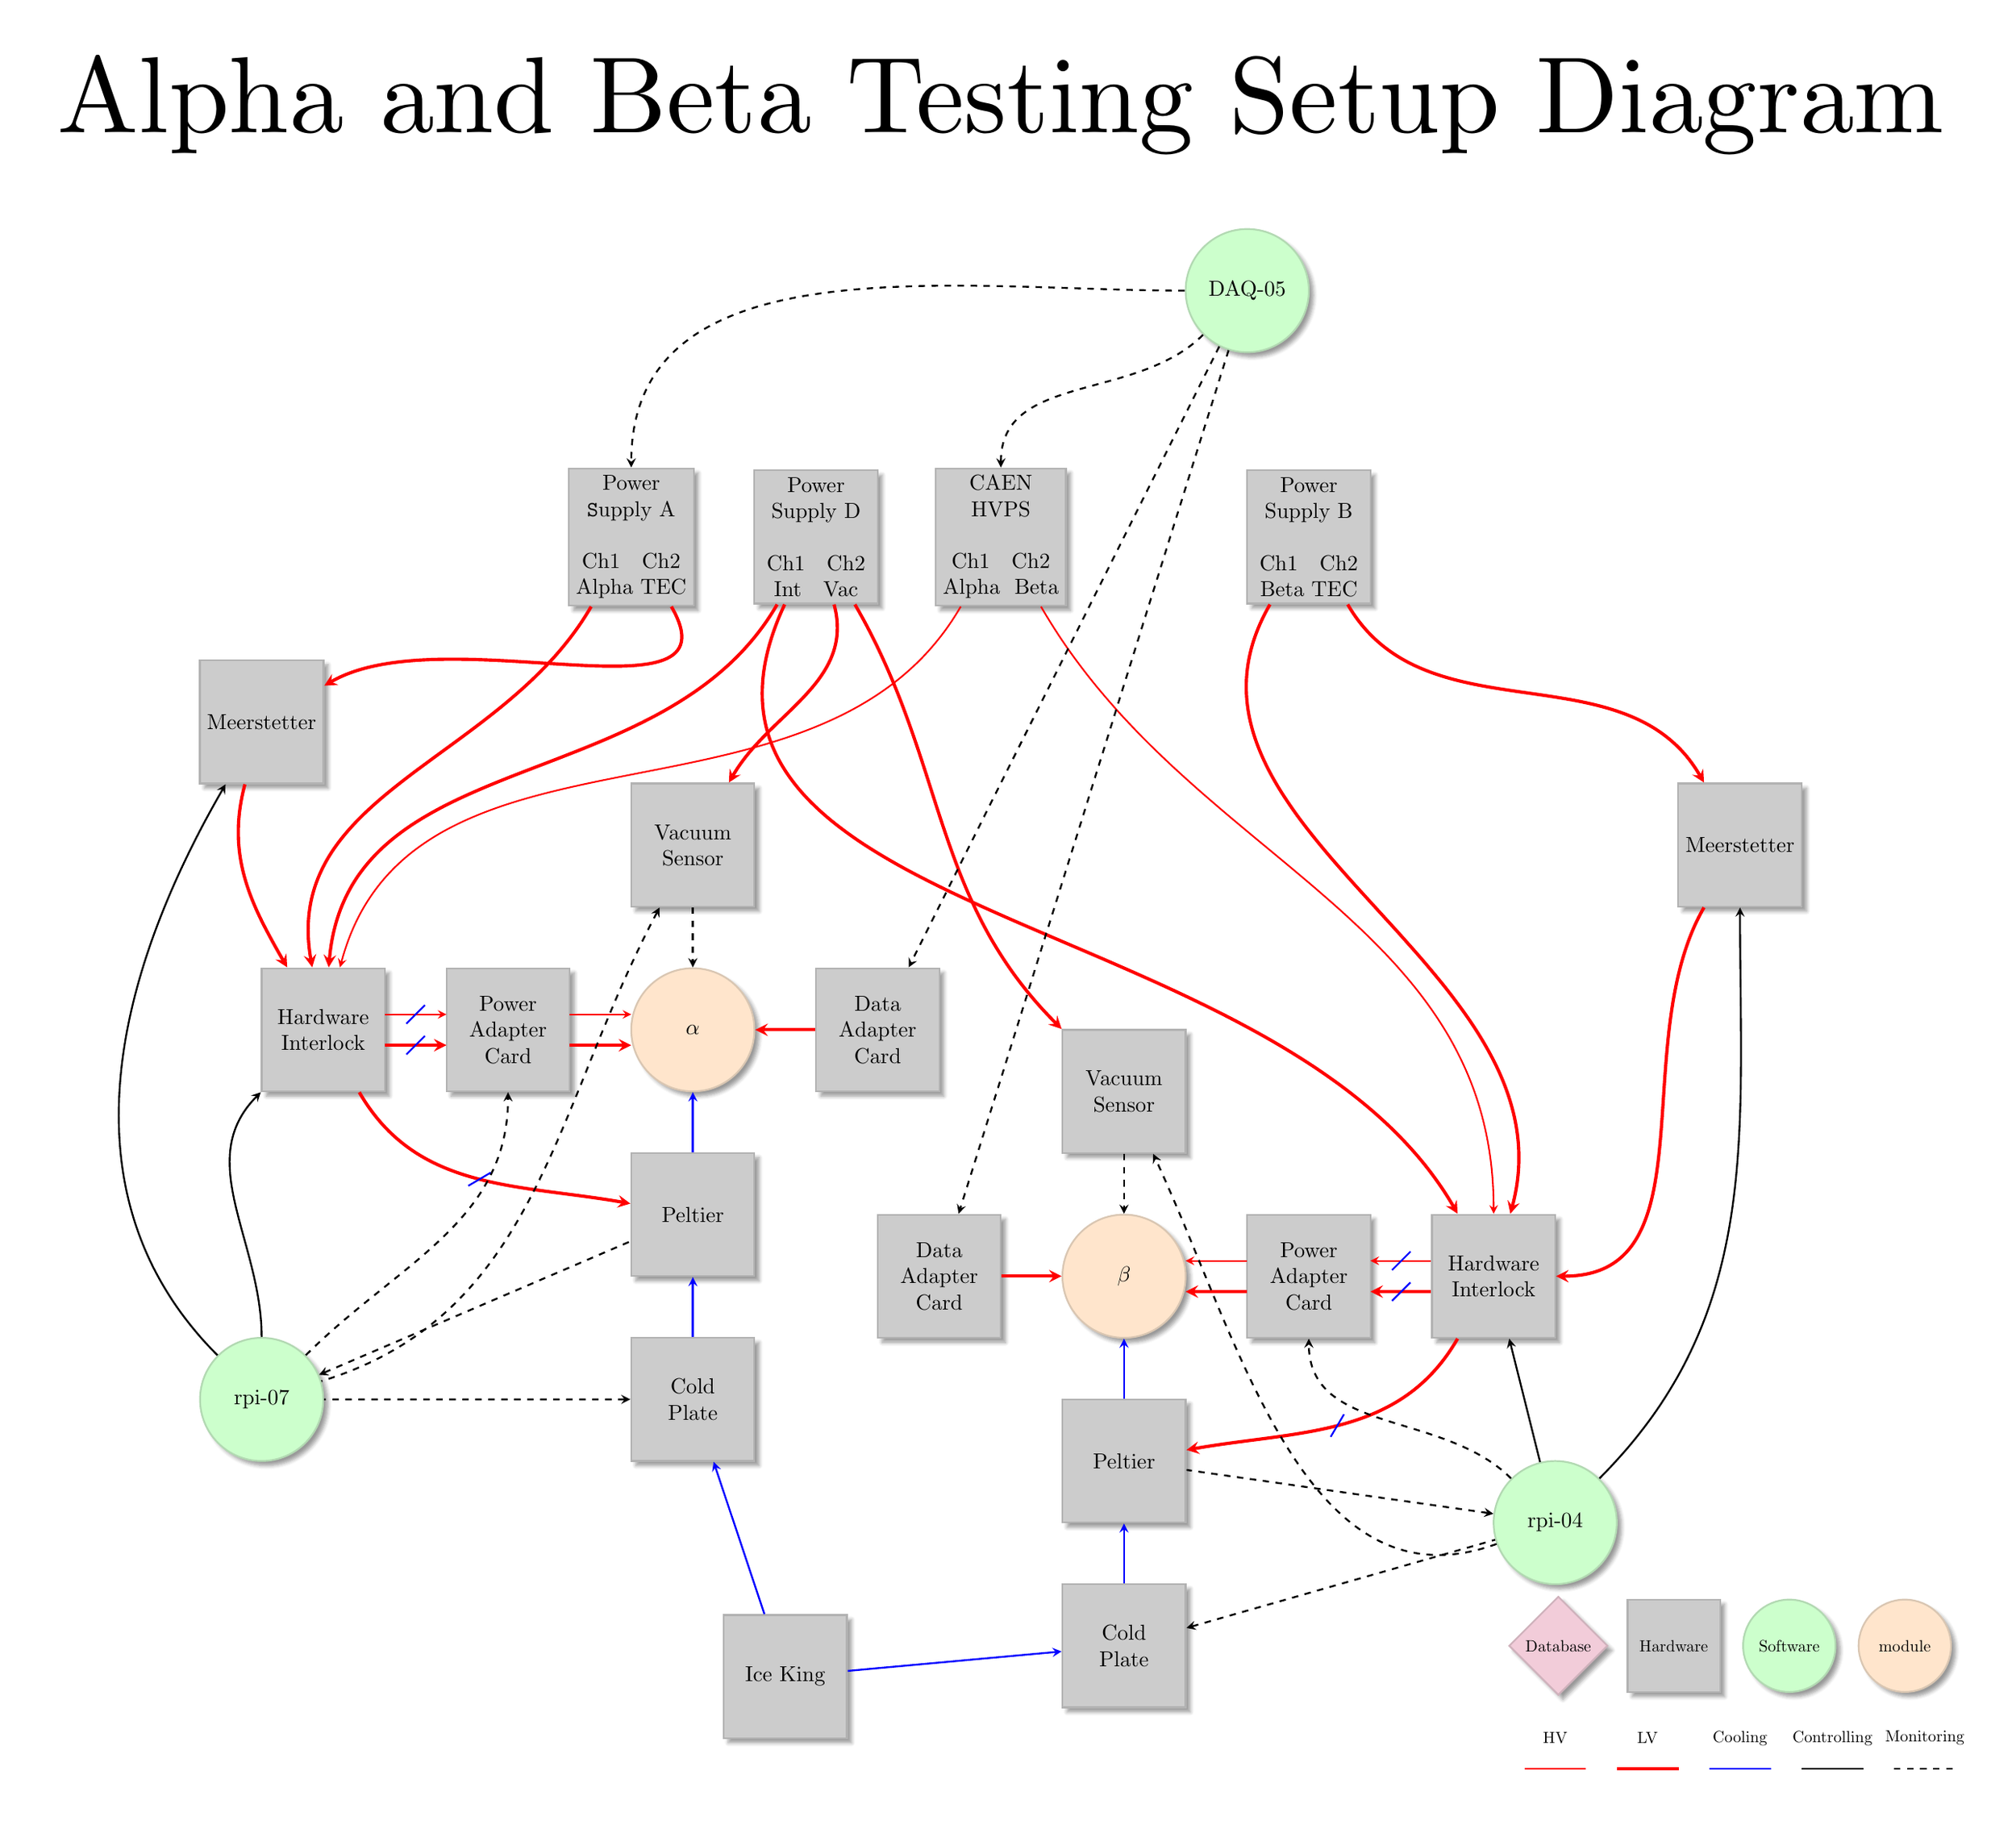
\begin{tikzpicture}[
	align=center,
        >=stealth,
        node distance=3cm,
	auto,
	line width=0.3mm,
        colorit/.style={
      	draw=#1!50!black!30,
      	fill=#1!20,
      	thick,
		blur shadow={shadow blur steps=5}
        },
        colorit/.default=black,
        database/.style={square, colorit=grey, shape border rotate=90, aspect=0.25, minimum size=2cm},
        software/.style={circle,colorit=green, minimum size=2cm},
	hardware/.style={rectangle,colorit=black, minimum size=2cm},
	module/.style={circle,colorit=orange, minimum size=2cm},
	database/.style={diamond,colorit=purple, minimum size=2cm},
	boxit/.style={
    	draw=#1!50!black!30,
		fill=#1!5,
		densely dotted,
		line width=0.5mm,
		rounded corners
	},
	boxit/.default=yellow
  	]
    %alpha beta set up
    \node[hardware] (psa) {Power\\\texttt Supply A\\\texttt {}\\\texttt {}Ch1 { { }}Ch2\\\texttt{}Alpha TEC};
    \node[hardware, right of = psa] (psd) {Power\\\texttt {}Supply D\\\texttt{}\\\texttt {}Ch1 { { }}Ch2\\\texttt{}Int { { }}Vac};
    \node[hardware, right of = psd] (hvps) {CAEN\\\texttt {}HVPS\\\texttt {}\\\texttt {}Ch1 { { }}Ch2\\\texttt{}Alpha{ } Beta};
    \node[hardware] at (11,0) (psb) {Power\\\texttt {}Supply B\\\texttt {}\\\texttt {}Ch1 { { }}Ch2\\\texttt{}Beta TEC};
    \node[hardware] at (-5,-8) (inta) {Hardware\\\texttt {}Interlock}
    edge[<-, red, line width= 1.5, in = 240, out = 100] (psa)
    edge[<-, red, line width= .75, in = 240, out = 75] (hvps)
    edge[<-, red, line width = 1.5, in = 240, out = 85] (psd);
    \node[hardware] at (-6,-3) (meera) {Meerstetter}
    edge[<-, red, line width = 1.5, in = 300, out = 30] (psa)
    edge[->, red, line width = 1.5, in = 120, out = 255] (inta);
    \node[hardware, right of = inta] (paca) {Power\\\texttt{}Adapter\\\texttt{}Card};
    \draw[->, red, line width=.75, strike thru arrow] (-4,-7.75) -- (-3,-7.75);
    \draw[->, red, line width=1.5, strike thru arrow] (-4,-8.25) -- (-3,-8.25);
    \node[module, right of = paca] (alpha) {$\alpha$};
    \draw[->, red, line width=.75] (-1,-7.75) -- (0,-7.75);
    \draw[->, red, line width=1.5] (-1,-8.25) -- (0,-8.25);
    \node[hardware, below of = alpha] (pelta) {Peltier}
    edge[<-, red, line width = 1.5, in = 300, out = 170, strike thru arrow] (inta)
    edge[->, blue] (alpha);
    \node[hardware, right of = alpha] (daca) {Data\\\texttt{}Adapter\\\texttt{}Card}
    edge[->, red, line width = 1.5] (alpha);
    \node[software] at (-6,-14) (rpi7) {rpi-07}
    edge[->, in = 225, out = 90] (inta)
    edge[->, in = 240, out = 135] (meera)
    edge[->, dashed, in = 270, out = 45] (paca)
    edge[<-, dashed] (pelta);
    \node[hardware, above of = alpha] (vac) {Vacuum\\\texttt{}Sensor}
    edge[<-, red, line width = 1.5, in = 285, out = 60] (psd)
    edge[->, dashed] (alpha)
    edge[<-, dashed, in = 17, out = 242] (rpi7);
    \node[module] at (8,-12) (beta) {$\beta$};
    \node[hardware, left of = beta] (dacb) {Data\\\texttt{}Adapter\\\texttt{}Card}
    edge[->, red, line width = 1.5](beta);
    \node[hardware, right of = beta] (pacb) {Power\\\texttt{}Adapter\\\texttt{}Card};
    \draw[<-, red, line width=.75] (9,-11.75) -- (10,-11.75);
    \draw[<-, red, line width=1.5] (9,-12.25) -- (10,-12.25);
    \draw[<-, red, line width=.75, strike thru arrow] (12,-11.75) -- (13,-11.75);
    \draw[<-, red, line width=1.5, strike thru arrow] (12,-12.25) -- (13,-12.25);
    \node[hardware, right of = pacb] (intb) {Hardware\\\texttt{}Interlock}
    edge[<-, red, line width = .75, in = 300, out = 90] (hvps)
    edge[<-, red, line width = 1.5, in = 240, out = 75] (psb)
    edge[<-, red, line width = 1.5, in = 245, out = 120] (psd);
    \node[hardware, below of = beta] (peltb) {Peltier}
    edge[->, blue](beta)
    edge[<-, red, line width = 1.5, out = 10, in = 240, strike thru arrow] (intb);
    \node[hardware, above of = beta] (vacb) {Vacuum\\\texttt{}Sensor}
    edge[->, dashed] (beta)
    edge[<-, red, line width = 1.5, in = 300, out = 135] (psd);
    \node[hardware] at (18, -5) (meerb) {Meerstetter}
    edge[<-, red, line width = 1.5, in = 300, out = 120] (psb)
    edge[->, red, line width = 1.5, in = 0, out = 240] (intb);
    \node[software] at (15,-16) (rpi4) {rpi-04}
    edge[->, in = 270, out = 45] (meerb)
    edge[->] (intb)
    edge[->, dashed, in = 270, out = 135] (pacb)
    edge[->, dashed, in = 295, out = 200] (vacb)
    edge[<-, dashed] (peltb);
    \node[software] at (10, 4) (daq5) {DAQ-05}
    edge[->, dashed] (daca)
    edge[->, dashed] (dacb)
    edge[->, dashed, in = 90, out = 180] (psa)
    edge[->, dashed, in = 90, out = 225] (hvps);
    \node[hardware, below of = pelta] (colda) {Cold\\\texttt{}Plate}
    edge[->, blue] (pelta)
    edge[<-, dashed] (rpi7);
    \node[hardware, below of = peltb] (coldb) {Cold\\\texttt{}Plate}
    edge[->, blue] (peltb)
    edge[<-, dashed] (rpi4);
    \node[hardware] at (2.5,-18.5) (chill) {Ice King}
    edge[->, blue] (colda)
    edge[->, blue] (coldb);
    \node at (0,-20.5) (blank) { };
    \node at (22,0) (blank) { };
    \node at (0,6) (blank) { };

\begin{scope}[every node/.append style={scale=5}, node distance=2.5cm]
    \node at (6,7) {Alpha and Beta Testing Setup Diagram};
\end{scope}
\begin{scope}[every node/.append style={scale=.75}, node distance=2.5cm]
    \node[database] (legend db) at (15.05,-18) {Database};
    \node[hardware, right of=legend db] (legend hw) {Hardware};
    \node[software, right of=legend hw] (legend sw) {Software};
    \node[module, right of=legend sw] (legend module) {module};
\end{scope}
\begin{scope}[every node/.append style={scale=.75}, node distance=2cm]
    \node (legend db) at (15,-19.5) {HV};
    \node[right of=legend db] (legend hw) {LV};
    \node[right of=legend hw] (legend sw) {Cooling};
    \node[right of=legend sw] (legend module) {Controlling};
    \node[right of=legend module] {Monitoring};
    \draw[-, red, line width = 0.75] (14.5,-20) -- (15.5,-20);
    \draw[-, red, line width=1.5pt] (16,-20) -- (17,-20);
    \draw[-, blue] (17.5,-20) -- (18.5,-20);
    \draw[-] (19,-20) -- (20,-20);
    \draw[-, dashed](20.5,-20) -- (21.5,-20);
\end{scope}
\end{tikzpicture}
\end{document}
